\documentclass[12pt,t]{beamer}
\usepackage{graphicx}
\setbeameroption{hide notes}
\setbeamertemplate{note page}[plain]

% get rid of junk
\usetheme{default}
\beamertemplatenavigationsymbolsempty
\hypersetup{pdfpagemode=UseNone} % don't show bookmarks on initial view

% font
\usepackage{fontspec}
\setsansfont{TeX Gyre Heros}
\setbeamerfont{note page}{family*=pplx,size=\footnotesize} % Palatino for notes
% "TeX Gyre Heros can be used as a replacement for Helvetica"
% In Unix, unzip the following into ~/.fonts
% In Mac, unzip it, double-click the .otf files, and install using "FontBook"
%   http://www.gust.org.pl/projects/e-foundry/tex-gyre/heros/qhv2.004otf.zip

% named colors
\definecolor{offwhite}{RGB}{249,242,215}
% \definecolor{foreground}{RGB}{255,255,255}
\definecolor{foreground}{RGB}{0,0,0}
% \definecolor{background}{RGB}{24,24,24}
\definecolor{background}{RGB}{255,255,255}
\definecolor{title}{RGB}{107,174,214}
\definecolor{gray}{RGB}{100,100,100}
\definecolor{subtitle}{RGB}{102,255,204}
\definecolor{hilight}{RGB}{20,180,204}
\definecolor{vhilight}{RGB}{255,111,207}
\definecolor{lolight}{RGB}{155,155,155}
%\definecolor{green}{RGB}{125,250,125}

% use those colors
\setbeamercolor{titlelike}{fg=title}
\setbeamercolor{subtitle}{fg=subtitle}
\setbeamercolor{institute}{fg=gray}
\setbeamercolor{normal text}{fg=foreground,bg=background}
\setbeamercolor{item}{fg=foreground} % color of bullets
\setbeamercolor{subitem}{fg=gray}
\setbeamercolor{itemize/enumerate subbody}{fg=gray}
\setbeamertemplate{itemize subitem}{{\textendash}}
\setbeamerfont{itemize/enumerate subbody}{size=\footnotesize}
\setbeamerfont{itemize/enumerate subitem}{size=\footnotesize}

% settings for table of contents
\setbeamercolor{section in toc}{fg=foreground,bg=background}
\setbeamerfont{subsection in toc}{size=\footnotesize}
\setbeamertemplate{section in toc}{{\scriptsize\leavevmode\raise1.35pt\hbox{$\blacktriangleright$}} \inserttocsection}
%\setbeamertemplate{subsection in toc}{\quad{\tiny\leavevmode\raise1.5pt\hbox{$\blacktriangleright$}} \footnotesize\inserttocsubsection\\}
\setbeamertemplate{subsection in toc}{\quad\quad\textendash\enspace\inserttocsubsection\\}

% page number
\setbeamertemplate{footline}{%
    \raisebox{5pt}{\makebox[\paperwidth]{\hfill\makebox[20pt]{\color{gray}
          \scriptsize\insertframenumber}}}\hspace*{5pt}}

% add a bit of space at the top of the notes page
\addtobeamertemplate{note page}{\setlength{\parskip}{12pt}}

% add subsection as frame title when it is empty
\makeatletter
  \CheckCommand*\beamer@checkframetitle{%
    \@ifnextchar\bgroup\beamer@inlineframetitle{}}
  \renewcommand*\beamer@checkframetitle{%
    \global\let\beamer@frametitle\relax\@ifnextchar%
    \bgroup\beamer@inlineframetitle{}}
\makeatother

\addtobeamertemplate{frametitle}{
  \ifx\insertframetitle\empty
      \frametitle{\insertsubsectionhead}
  \else
  \fi
 }{}

% a few macros
\newcommand{\bi}{\begin{itemize}}
\newcommand{\ei}{\end{itemize}}
\newcommand{\ig}{\includegraphics}
\newcommand{\subt}[1]{{\footnotesize \color{subtitle} {#1}}}


% title info
\title{Geometry}
\author{Gregor Behnke}
\institute{Institute of Artificial Intelligence\\ Ulm University}
\date{\tiny based on Bjarki Ágúst Guðmundsson's and Tómas Ken Magnússon's\\Competitive Programming}
% \date{\href{http://www.biostat.wisc.edu/~kbroman}{\tt \scriptsize biostat.wisc.edu/{\textasciitilde}kbroman}
% \\[-4pt]
% \href{http://github.com/kbroman}{\tt \scriptsize github.com/kbroman}
% }



% Tikz
\usepackage{tikz}
\usepackage{tkz-euclide}
% \usepackage{intersections}
\usetkzobj{all}
\usetikzlibrary{arrows,shapes,angles,quotes,shapes, calc, decorations}

% Minted
\usepackage{minted}
\usemintedstyle{tango}
\newminted{cpp}{fontsize=\footnotesize}

% Graph styles
\tikzstyle{vertex}=[circle,fill=black!50,minimum size=15pt,inner sep=0pt, font=\small]
\tikzstyle{selected vertex} = [vertex, fill=red!24]
\tikzstyle{edge} = [draw,thick,-]
\tikzstyle{dedge} = [draw,thick,->]
\tikzstyle{weight} = [font=\scriptsize,pos=0.5]
\tikzstyle{selected edge} = [draw,line width=2pt,-,red!50]
\tikzstyle{ignored edge} = [draw,line width=5pt,-,black!20]


\begin{document}

% title slide
{
    \setbeamertemplate{footline}{} % no page number here
    \frame{
        \titlepage
    }
}

%\AtBeginSection[]
%{
  %\begin{frame}<beamer>{Geometry}
    %\vspace{20pt}
    %\tableofcontents[
      %currentsection,
      %hideallsubsections,
      %%currentsubsection,
      %%hideothersubsections,
      %sectionstyle=show/shaded%,
      %%subsectionstyle=show/shaded/hide
    %]
  %\end{frame}
%}

\begin{frame}<beamer>{Today we're going to cover}
    \vspace{40pt}
    %\tableofcontents[hideallsubsections]
    \bi
      \item Geometry
      \item Computational geometry \pause
      \item Only 2D-Geometry, 3D is similar just with one more dimension
    \ei
\end{frame}

\section{Geometry}
\subsection{Points and vectors}


\begin{frame}
  \begin{columns}
    \begin{column}{0.4\textwidth}
      \begin{figure}
        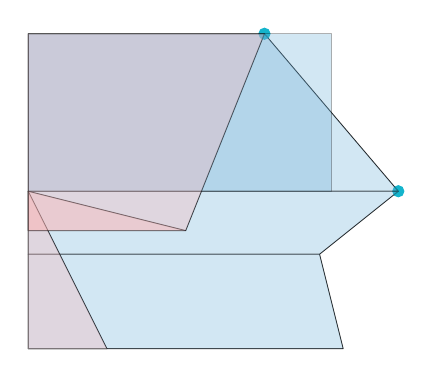
\begin{tikzpicture}
          \coordinate(A) at (0,0);
          \coordinate(B) at (3,0);
          \coordinate(C) at (2.7,1.2);
          \coordinate(D) at (3.7,2);
          \coordinate(E) at (2,4);
          \coordinate(F) at (1,1.5);
          \coordinate(G) at (-1,2);

          \coordinate(Dm) at (2.85,2);
          \coordinate(Em) at (2.85,4);

          \coordinate(Ap) at (-1,0);
          \coordinate(Bp) at (-1,0);
          \coordinate(Cp) at (-1,1.2);
          \coordinate(Dp) at (-1,2);
          \coordinate(Ep) at (-1,4);
          \coordinate(Fp) at (-1,1.5);
          \coordinate(Gp) at (-1,2);

          \tkzDrawPolygon[color=foreground](A,B,C,D,E,F,G);

          \visible<3-5>{
            \draw[fill,hilight] (E) circle[radius=2pt];
            \draw[fill,hilight] (D) circle[radius=2pt];
          }

          \visible<4>{\tkzDrawPolygon[color=foreground,fill=title,opacity=0.3,thin](E,D,Dp,Ep);}
          \visible<5>{\tkzDrawPolygon[color=foreground,fill=title,opacity=0.3,thin](Em,Dm,Dp,Ep);}
          \visible<6>{\tkzDrawPolygon[color=foreground,fill=title,opacity=0.3,thin](D,C,Cp,Dp);}
          \visible<7>{\tkzDrawPolygon[color=foreground,fill=title,opacity=0.3,thin](C,B,Bp,Cp);}
          \visible<8>{\tkzDrawPolygon[color=foreground,fill=red!30,opacity=0.3,thin](A,G,Gp,Ap);}
          \visible<9>{\tkzDrawPolygon[color=foreground,fill=red!30,opacity=0.3,thin](G,F,Fp,Gp);}
          \visible<10>{\tkzDrawPolygon[color=foreground,fill=red!30,opacity=0.3,thin](F,E,Ep,Fp);}
        \end{tikzpicture}
      \end{figure}
    \end{column}
    \begin{column}{0.6\textwidth}
      \bi
        \item Polygons are represented by a list of points in the order
          representing the edges.
        \onslide<2->
        \item To calculate the area
          \bi
            \onslide<3->
            \item Go clockwise through all edges of the polygon 
            \onslide<4->
            \item Calculate the area of the polygone whose other side is the y-axis\only<5->{, by computing the area of the respective rectangle}
            \onslide<8->
            \item Top-Down and Bottom-Up edges cancel the area outside the polygon out.
          \ei
      \ei
    \end{column}
  \end{columns}
\end{frame}
\end{document}

